%%%%%%%%%%%%%%%%%%%%%%%%%%%%%%%%%%%%%%%%%
% Short Sectioned Assignment
% LaTeX Template
% Version 1.0 (5/5/12)
%
% This template has been downloaded from:
% http://www.LaTeXTemplates.com
%
% Original author:
% Frits Wenneker (http://www.howtotex.com)
%
% License:
% CC BY-NC-SA 3.0 (http://creativecommons.org/licenses/by-nc-sa/3.0/)
%
%%%%%%%%%%%%%%%%%%%%%%%%%%%%%%%%%%%%%%%%%

%----------------------------------------------------------------------------------------
%	PACKAGES AND OTHER DOCUMENT CONFIGURATIONS
%----------------------------------------------------------------------------------------

\documentclass[paper=a4, fontsize=11pt]{scrartcl} % A4 paper and 11pt font size

\usepackage[T1]{fontenc} % Use 8-bit encoding that has 256 glyphs
\usepackage{fourier} % Use the Adobe Utopia font for the document - comment this line to return to the LaTeX default
\usepackage[english]{babel} % English language/hyphenation
\usepackage{amsmath,amsfonts,amsthm} % Math packages

\usepackage{graphicx}

\usepackage{sectsty} % Allows customizing section commands
\allsectionsfont{\centering \normalfont\scshape} % Make all sections centered, the default font and small caps

\usepackage[procnames]{listings}

\usepackage{fancyhdr} % Custom headers and footers
\pagestyle{fancyplain} % Makes all pages in the document conform to the custom headers and footers
\fancyhead{} % No page header - if you want one, create it in the same way as the footers below
\fancyfoot[L]{} % Empty left footer
\fancyfoot[C]{} % Empty center footer
\fancyfoot[R]{\thepage} % Page numbering for right footer
\renewcommand{\headrulewidth}{0pt} % Remove header underlines
\renewcommand{\footrulewidth}{0pt} % Remove footer underlines
\setlength{\headheight}{13.6pt} % Customize the height of the header

\numberwithin{equation}{section} % Number equations within sections (i.e. 1.1, 1.2, 2.1, 2.2 instead of 1, 2, 3, 4)
\numberwithin{figure}{section} % Number figures within sections (i.e. 1.1, 1.2, 2.1, 2.2 instead of 1, 2, 3, 4)
\numberwithin{table}{section} % Number tables within sections (i.e. 1.1, 1.2, 2.1, 2.2 instead of 1, 2, 3, 4)

\setlength\parindent{0pt} % Removes all indentation from paragraphs - comment this line for an assignment with lots of text

%----------------------------------------------------------------------------------------
%	TITLE SECTION
%----------------------------------------------------------------------------------------

\newcommand{\horrule}[1]{\rule{\linewidth}{#1}} % Create horizontal rule command with 1 argument of height

\title{	
\normalfont \normalsize 
\textsc{BRSU} \\ [25pt] % Your university, school and/or department name(s)
\horrule{0.5pt} \\[0.4cm] % Thin top horizontal rule
\huge Neural Networks\\Assignment 8 \\ % The assignment title
\horrule{2pt} \\[0.5cm] % Thick bottom horizontal rule
}

\author{Bastian Lang} % Your name

\date{\normalsize\today} % Today's date or a custom date

\begin{document}

\maketitle % Print the title

\newpage



\section{Exercise 5.10}

\subsection{Note}
This exercise does not make much sense if the other parameters are not given. If I would have chosen a very big radius, then the vertical separation would not have had any impact at all...

\subsection{output}
Figure \ref{figv1} till \ref{figvn6} show clustered data with variation of vertical separation.\\
One can observe that the clusters "mix", i.e. parts of the lower figure become part of clusters of the upper figure and vice versa.\\

This also effects the mean and the variance, but mostly in y-direction. The other figures show all means for the different clusters. I had to drop the variance figures because of technical problems and no time left while building the pdf...


\begin{figure}[ht]
	\centering
  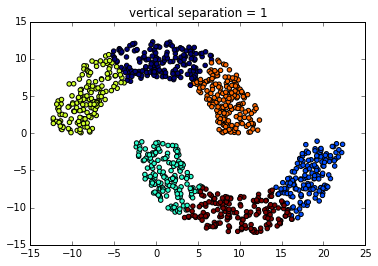
\includegraphics[width=0.8\textwidth]{v1.png}
	\caption{Clustered samples from figure with vertical separation of 1}
	\label{figv1}
\end{figure}

\begin{figure}[ht]
	\centering
  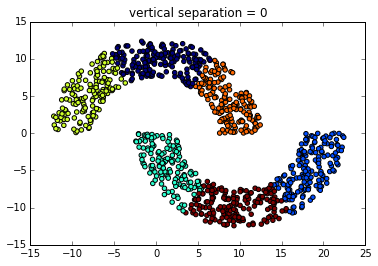
\includegraphics[width=0.8\textwidth]{v0.png}
	\caption{Clustered samples from figure with vertical separation of 0}
	\label{figv0}
\end{figure}

\begin{figure}[ht]
	\centering
  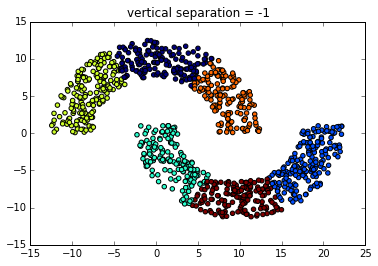
\includegraphics[width=0.8\textwidth]{vn1.png}
	\caption{Clustered samples from figure with vertical separation of -1}
	\label{figvn1}
\end{figure}
\begin{figure}[ht]
	\centering
  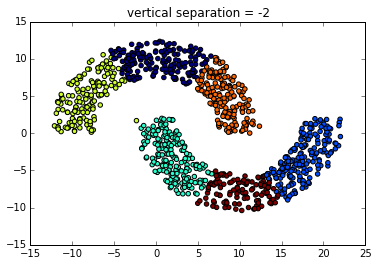
\includegraphics[width=0.8\textwidth]{vn2.png}
	\caption{Clustered samples from figure with vertical separation of -2}
	\label{figvn2}
\end{figure}
\begin{figure}[ht]
	\centering
  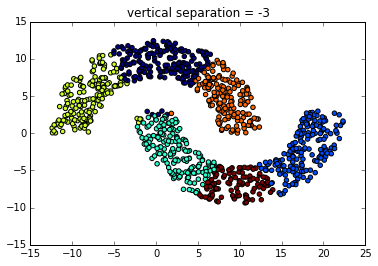
\includegraphics[width=0.8\textwidth]{vn3.png}
	\caption{Clustered samples from figure with vertical separation of -3}
	\label{figvn3}
\end{figure}
\begin{figure}[ht]
	\centering
  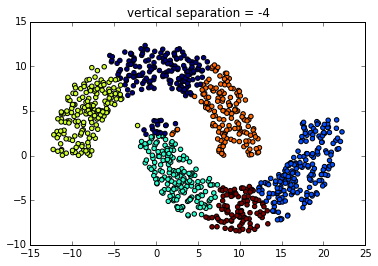
\includegraphics[width=0.8\textwidth]{vn4.png}
	\caption{Clustered samples from figure with vertical separation of -4}
	\label{figvn4}
\end{figure}
\begin{figure}[ht]
	\centering
  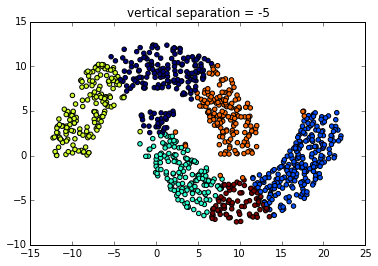
\includegraphics[width=0.8\textwidth]{vn5.png}
	\caption{Clustered samples from figure with vertical separation of -5}
	\label{figvn5}
\end{figure}
\begin{figure}[ht]
	\centering
  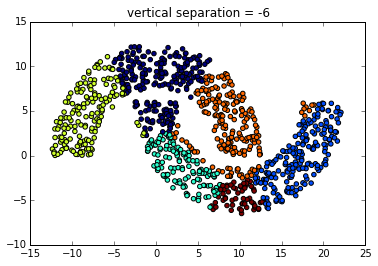
\includegraphics[width=0.8\textwidth]{vn6.png}
	\caption{Clustered samples from figure with vertical separation of -6}
	\label{figvn6}
\end{figure}


\begin{figure}[ht]
	\centering
  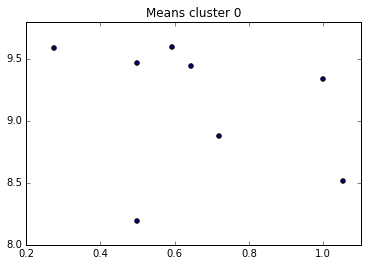
\includegraphics[width=0.8\textwidth]{mean_c1.png}
	\caption{Means of cluster 1}
	\label{figvn6}
\end{figure}
\begin{figure}[ht]
	\centering
  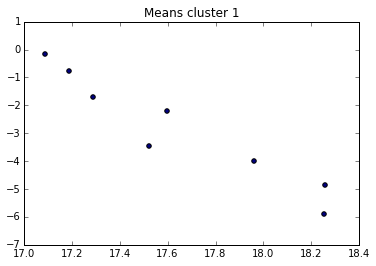
\includegraphics[width=0.8\textwidth]{mean_c2.png}
	\caption{Means of cluster 2}
	\label{figvn6}
\end{figure}
\begin{figure}[ht]
	\centering
  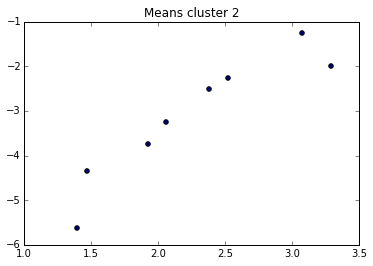
\includegraphics[width=0.8\textwidth]{mean_c3.png}
	\caption{Means of cluster 3}
	\label{figvn6}
\end{figure}
\begin{figure}[ht]
	\centering
  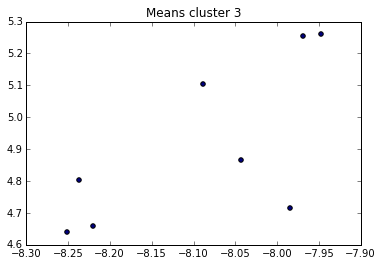
\includegraphics[width=0.8\textwidth]{mean_c4.png}
	\caption{Means of cluster 4}
	\label{figvn6}
\end{figure}
\begin{figure}[ht]
	\centering
  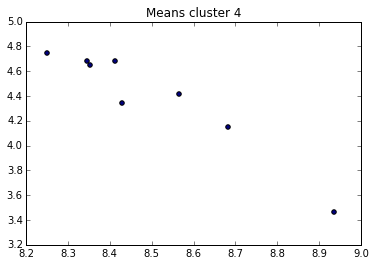
\includegraphics[width=0.8\textwidth]{mean_c5.png}
	\caption{Means of cluster 5}
	\label{figvn6}
\end{figure}
\begin{figure}[ht]
	\centering
  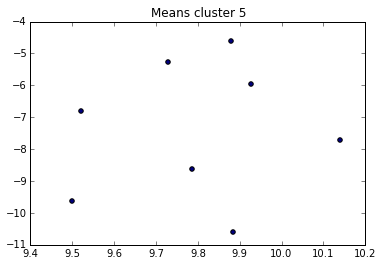
\includegraphics[width=0.8\textwidth]{mean_c6.png}
	\caption{Means of cluster 6}
	\label{figvn6}
\end{figure}

\begin{figure}[ht]
	\centering
  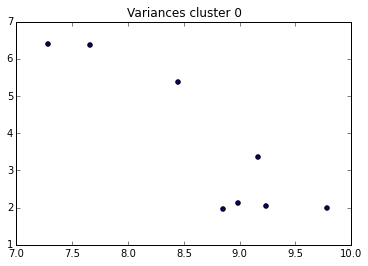
\includegraphics[width=0.8\textwidth]{variance_c1.png}
	\caption{Variances of cluster 1}
	\label{figv1}
\end{figure}
\begin{figure}[ht]
	\centering
  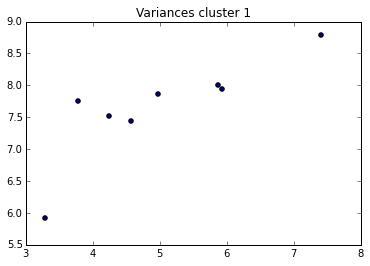
\includegraphics[width=0.8\textwidth]{variance_c2.png}
	\caption{Variances of cluster 2}
	\label{figv2}
\end{figure}
\begin{figure}[ht]
	\centering
  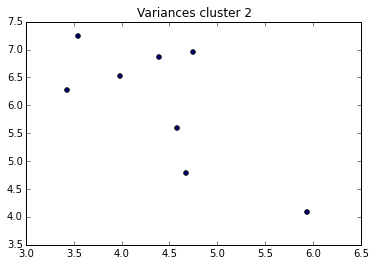
\includegraphics[width=0.8\textwidth]{variance_c3.png}
	\caption{Variances of cluster 3}
	\label{figv3}
\end{figure}
\begin{figure}[ht]
	\centering
  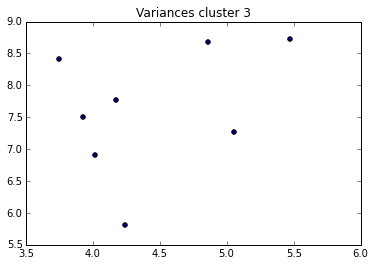
\includegraphics[width=0.8\textwidth]{variance_c4.png}
	\caption{Variances of cluster 4}
	\label{figv4}
\end{figure}

\begin{figure}[ht]
	\centering
  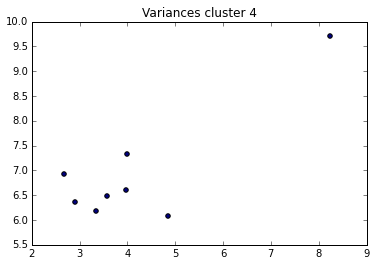
\includegraphics[width=0.8\textwidth]{variance_c5.png}
	\caption{Variances of cluster 5}
	\label{figv5}
\end{figure}

\begin{figure}[ht]
	\centering
  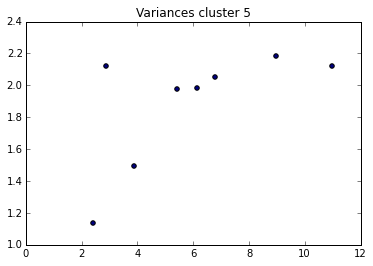
\includegraphics[width=0.8\textwidth]{variance_c6.png}
	\caption{Variances of cluster 6}
	\label{figv6}
\end{figure}


\subsection{code}
\begin{lstlisting}
# -*- coding: utf-8 -*-
"""
Created on Sat Nov 28 14:24:39 2015

@author: bastian
"""

import random
import numpy as np
from matplotlib import pyplot as plt
from sklearn.cluster import KMeans


RADIUS = 10
WIDTH = 5
VERTICAL_SEPARATION = 5

def sample_upper_halfmoon(radius, width):
    distance = random.random() * width + radius - 0.5 * width
    angle = random.random() * 180
    angle = np.radians(angle)
    x = np.cos(angle) * distance
    y = np.sin(angle) * distance
    return x,y
    
def sample_lower_halfmoon(radius, width, vertical_separation):
    distance = random.random() * width + radius - 0.5 * width
    angle = random.random() * 180 + 180
    angle = np.radians(angle)
    x = np.cos(angle) * distance + radius
    y = np.sin(angle) * distance - vertical_separation
    return x,y
    
def sample_figure(radius, width, vertical_separation):
    index = random.randint(0,1)
    if(index == 0):
        return sample_upper_halfmoon(radius, width)
    else:
        return sample_lower_halfmoon(radius, width, vertical_separation)
        
def sample_and_cluster(radius, width, vertical_separation):
    X = []
    Y = []
    points = [] 
    for i in range (1000):
        x,y = sample_figure(radius, width, vertical_separation)
        X.append(x)
        Y.append(y)
        points.append([x,y])
    
    kmeans = KMeans(n_clusters = 6)
    kmeans.fit(points)
    labels = kmeans.labels_
    fig1 = plt.figure()
    plt.title('vertical separation = '+ str(vertical_separation))
    ax1 = fig1.add_subplot(111)
    ax1.scatter(X, Y, c=labels.astype(np.float))
    
    c1=[]
    c2=[]
    c3=[]
    c4=[]
    c5=[]
    c6=[]
    for i in range(len(labels)):
        cluster = labels[i]
        point = points[i]
        if(cluster == 0):
            c1.append(point)
        elif(cluster == 1):
            c2.append(point)
        elif(cluster == 2):
            c3.append(point)
        elif(cluster == 3):
            c4.append(point)
        elif(cluster == 4):
            c5.append(point)
        elif(cluster == 5):
            c6.append(point)
    return c1,c2,c3,c4,c5,c6

def get_clusters(data, labels):
    c1=[]
    c2=[]
    c3=[]
    c4=[]
    c5=[]
    c6=[]
    for i in range(len(labels)):
        cluster = labels[i]
        point = data[i]
        if(cluster == 0):
            c1.append(point)
        elif(cluster == 1):
            c2.append(point)
        elif(cluster == 2):
            c3.append(point)
        elif(cluster == 3):
            c4.append(point)
        elif(cluster == 4):
            c5.append(point)
        elif(cluster == 5):
            c6.append(point)
    return c1,c2,c3,c4,c5,c6

def plot_data(data, title):
    fig = plt.figure()
    plt.title(title)
    ax = fig.add_subplot(111)
    x,y = get_x_y_values(data)    
    ax.scatter(x, y)
          
def vary_vertical_separation():
    c1_means = []
    c2_means = []
    c3_means = []
    c4_means = []
    c5_means = []
    c6_means = []
    c1_variances = []
    c2_variances = []
    c3_variances = []
    c4_variances = []
    c5_variances = []
    c6_variances = []
    for i in range(-6,2):
        c1,c2,c3,c4,c5,c6 = sample_and_cluster(RADIUS,WIDTH,i)
        mean_1 = compute_mean(c1)
        c1_means.append(mean_1)
        c1_variances.append(compute_variance(c1, mean_1))
        mean_2 = compute_mean(c2)
        c2_means.append(mean_2)
        c2_variances.append(compute_variance(c2, mean_2))
        mean_3 = compute_mean(c3)
        c3_means.append(mean_3)
        c3_variances.append(compute_variance(c3, mean_3))
        mean_4 = compute_mean(c4)
        c4_means.append(mean_4)
        c4_variances.append(compute_variance(c4, mean_4))
        mean_5 = compute_mean(c5)
        c5_means.append(mean_5)
        c5_variances.append(compute_variance(c5, mean_5))
        mean_6 = compute_mean(c6)
        c6_means.append(mean_6)
        c6_variances.append(compute_variance(c6, mean_6))
    
    fig = plt.figure()
    plt.title('means of cluster 1')
    ax = fig.add_subplot(111)
    x,y = get_x_y_values(c1_means)    
    ax.scatter(x, y)
    
    fig = plt.figure()
    plt.title('means of cluster 2')
    ax = fig.add_subplot(111)
    x,y = get_x_y_values(c2_means)    
    ax.scatter(x, y)
    
    fig = plt.figure()
    plt.title('means of cluster 3')
    ax = fig.add_subplot(111)
    x,y = get_x_y_values(c3_means)    
    ax.scatter(x, y)    

    fig = plt.figure()
    plt.title('means of cluster 4')
    ax = fig.add_subplot(111)
    x,y = get_x_y_values(c4_means)    
    ax.scatter(x, y)

    fig = plt.figure()
    plt.title('means of cluster 5')    
    ax = fig.add_subplot(111)
    x,y = get_x_y_values(c5_means) 
    ax.scatter(x, y)

    fig = plt.figure()
    plt.title('means of cluster 6')    
    ax = fig.add_subplot(111)
    x,y = get_x_y_values(c6_means)    
    ax.scatter(x, y)   
    
    fig = plt.figure()
    plt.title('variances of cluster 1')
    ax = fig.add_subplot(111)
    x,y = get_x_y_values(c1_variances)    
    ax.scatter(x, y)
    
    fig = plt.figure()
    plt.title('variances of cluster 2')
    ax = fig.add_subplot(111)
    x,y = get_x_y_values(c2_variances)    
    ax.scatter(x, y)

    fig = plt.figure()
    plt.title('variances of cluster 3')    
    ax = fig.add_subplot(111)
    x,y = get_x_y_values(c3_variances)    
    ax.scatter(x, y)    

    fig = plt.figure()
    plt.title('variances of cluster 4')
    ax = fig.add_subplot(111)
    x,y = get_x_y_values(c4_variances)    
    ax.scatter(x, y)

    fig = plt.figure()
    plt.title('variances of cluster 5')    
    ax = fig.add_subplot(111)
    x,y = get_x_y_values(c5_variances) 
    ax.scatter(x, y)

    fig = plt.figure()
    plt.title('variances of cluster 6')    
    ax = fig.add_subplot(111)
    x,y = get_x_y_values(c6_variances)    
    ax.scatter(x, y) 

def get_x_y_values(data):
    x = []
    y = []
    for point in data:
        x.append(point[0])
        y.append(point[1])
    return x,y
        
        
def compute_mean(data):
    mean = [0,0]
    for point in data:
        mean[0] += point[0]
        mean[1] += point[1]
    return mean[0]/len(data), mean[1] / len(data)
    
def compute_variance(data, mean):
    sum_squared_differences = [0,0]
    for point in data:    
        squared_difference = ((point[0] - mean[0])**2, (point[1] - mean[1])**2)
        sum_squared_differences[0] += squared_difference[0]
        sum_squared_differences[1] += squared_difference[1]
        
    return sum_squared_differences[0]/len(data), sum_squared_differences[1] /len(data)

def compute_mean_and_variance_for_clusters(clusters):
    means = []
    variances = []
    for cluster in clusters:
        mean = compute_mean(cluster)
        means.append(mean)
        variances.append(compute_variance(cluster, mean))
    return means, variances
    

# Sample data points from figure
samples = []
for i in range(1000):
    samples.append(sample_figure(RADIUS, WIDTH, 0))
# Cluster data points using kmeans
X,Y = get_x_y_values(samples)
kmeans = KMeans(n_clusters = 6)
kmeans.fit(samples)
labels = kmeans.labels_
fig1 = plt.figure()
plt.title('vertical separation = 0')
ax1 = fig1.add_subplot(111)
ax1.scatter(X, Y, c=labels.astype(np.float))

# Sample data points for varying vertical separation
all_means = []
all_variances = []
for i in range(-6,2):
    samples = []
    for j in range(1000):
        samples.append(sample_figure(RADIUS, WIDTH, i))
    labels = kmeans.predict(samples)
    X,Y = get_x_y_values(samples)
    fig1 = plt.figure()
    plt.title('vertical separation = ' + str(i))
    ax1 = fig1.add_subplot(111)
    ax1.scatter(X, Y, c=labels.astype(np.float))
    
    clusters = get_clusters(samples, labels)
    means, variances = compute_mean_and_variance_for_clusters(clusters)
    all_means.append(means)
    all_variances.append(variances)

# Print means
for i in range(6):
    fig1 = plt.figure()
    plt.title('Means cluster ' + str(i))
    ax1 = fig1.add_subplot(111)    
    for mean in all_means:
        ax1.scatter(mean[i][0], mean[i][1], c= float(i) / 6.0 )
        
# Print variances
for i in range(6):
    fig1 = plt.figure()
    plt.title('Variances cluster ' + str(i))
    ax1 = fig1.add_subplot(111)    
    for variance in all_variances:
        ax1.scatter(variance[i][0], variance[i][1], c= float(i) / 6.0 )
    


\end{lstlisting}



\end{document}